
%% Harvard Physics Project
%% Test Booklet 3: The Triumph of Mechanics
%%--------------------------------------------------


%% Test Booklet 3 contains 70 - 6 - 4 questions


%% Test A
%%--------------------
\element{project}{
\begin{question}{testA-Q01}
    When the speed of a car is doubled, the car's:
    \begin{choices}
        \wrongchoice{kinetic energy is doubled. }
        \wrongchoice{potential energy is doubled. }
      \correctchoice{momentum is doubled. }
        \wrongchoice{acceleration is doubled. }
        \wrongchoice{inertia is doubled. }
    \end{choices}
\end{question}
}

\element{project}{
\begin{question}{testA-Q02}
    A freight car of mass \SI{2.0e4}{\kilo\gram} standing at rest
        is rammed by a loaded tank car with a mass of \SI{3.0e4}{\kilo\gram}.
    After the collision, the two cars are locked together and move
        off at a speed of \SI{0.60}{\meter\per\second}.
    What was the speed of the tank car before the collision?
    \begin{multicols}{2}
    \begin{choices}
        \wrongchoice{\SI{0.20}{\meter\per\second}}
        \wrongchoice{\SI{0.75}{\meter\per\second}}
      \correctchoice{\SI{1.0}{\meter\per\second}}
        \wrongchoice{\SI{3.6}{\meter\per\second}}
        \wrongchoice{\SI{4.0}{\meter\per\second}}
        %% NOTE: added one for symmetry
        %% NOTE: this is really good!!
        \wrongchoice{\SI{1.5}{\meter\per\second}}
    \end{choices}
    \end{multicols}
\end{question}
}

\element{project}{
\begin{question}{testA-Q03}
    When two waves pass the same point at the same time,
        their amplitudes at this point always:
    \begin{choices}
        \wrongchoice{cancel.}
        \wrongchoice{reflect off each other.}
        \wrongchoice{reinforce each other.}
        \wrongchoice{hinder each other's progress.}
      \correctchoice{superpose.}
    \end{choices}
\end{question}
}

\element{project}{
\begin{question}{testA-Q04}
    In a certain medium the speed of a group of waves has a fixed value.
    If the frequency of the waves is doubled, their wavelength will be:
    \begin{choices}
        \wrongchoice{4 times its original value.}
        \wrongchoice{2 times its original value.}
        \wrongchoice{unchanged.}
      \correctchoice{$\frac{1}{2}$ its original value.}
        \wrongchoice{$\frac{1}{4}$ its original value.}
    \end{choices}
\end{question}
}

\element{project}{
\begin{questionmult}{testA-Q05}
    Which of the following three quantities have the same magnitude
        just before and just after a perfectly elastic collision?
    \begin{choices}
      \correctchoice{momentum}
      \correctchoice{kinetic energy}
      %% NOTE: remove total energy?
      \correctchoice{total energy}
    \end{choices}
\end{questionmult}
}

\element{project}{
\begin{question}{testA-Q06}
    %Questions 6, 7, and 8
    Below are the names of scientists who made early
        significant contributions to the study of thermodynamics.
    Which statement best describe the contributions of James Prescott Joule?
    \begin{choices}
        \wrongchoice{The pressure of a gas is proportional to the square of the speed of its molecules.}
      \correctchoice{Heat is a form of energy.}
        \wrongchoice{The speeds of molecules in a gas follow a statistical law.}
        \wrongchoice{In an elastic collision, momentum is conserved.}
        \wrongchoice{The process of equalization of temperatures by the flow of heat from hot to cold bodies is always taking place in nature.}
    \end{choices}
\end{question}
}

\element{project}{
\begin{question}{testA-Q07}
    %Questions 6, 7, and 8
    Below are the names of scientists who made early
        significant contributions to the study of thermodynamics.
    Which statement best describe the contributions of
        Nicolas L\'{e}onard Sadi Carnot?
    \begin{choices}
        \wrongchoice{The pressure of a gas is proportional to the square of the speed of its molecules.}
        \wrongchoice{Heat is a form of energy.}
        \wrongchoice{The speeds of molecules in a gas follow a statistical law.}
        \wrongchoice{In an elastic collision, momentum is conserved.}
      \correctchoice{The process of equalization of temperatures by the flow of heat from hot to cold bodies is always taking place in nature.}
    \end{choices}
\end{question}
}

\element{project}{
\begin{question}{testA-Q08}
    Below are the names of scientists who made early
        significant contributions to the study of thermodynamics.
    Which statement best describe the contributions of
        James Clerk Maxwell?
    \begin{choices}
        \wrongchoice{The pressure of a gas is proportional to the square of the speed of its molecules.}
        \wrongchoice{Heat is a form of energy.}
      \correctchoice{The speeds of molecules in a gas follow a statistical law.}
        \wrongchoice{In an elastic collision, momentum is conserved.}
        \wrongchoice{The process of equalization of temperatures by the flow of heat from hot to cold bodies is always taking place in nature.}
    \end{choices}
\end{question}
}

\element{project}{
\begin{question}{testA-Q09}
    A girl lifts a bowling ball from the floor and places it on a rack.
    If you know the weight of the ball,
        what else must you know in order to calculate the work she does on the ball?
    \begin{choices}
        \wrongchoice{mass of the ball}
        %% NOTE: changed a_g to g
        \wrongchoice{value of $g$}
      \correctchoice{height of the rack}
        \wrongchoice{the time required}
        \wrongchoice{nothing else}
    \end{choices}
\end{question}
}

\begin{comment}
\newcommand{\projectTestAQTen}{
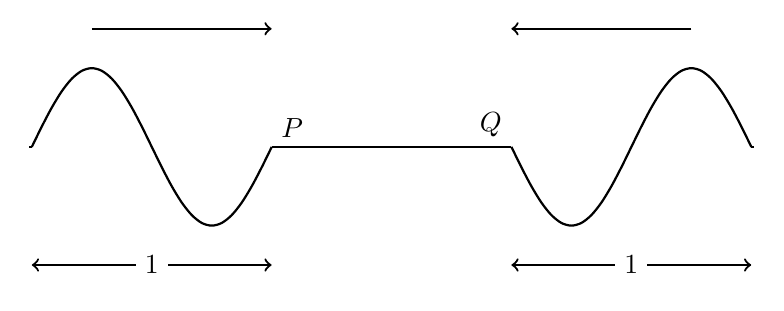
\begin{tikzpicture}[x=0.04\columnwidth]
    %% left
    \draw[thick] (0,0) -- (-3.14,0);
    \draw[domain=0:2*pi,smooth,thick] plot (\x-9.42, {1*sin(\x r)});
    \draw[thick] (-9.42,0) -- (-9.50,0);
    \draw[thick,->] (-7.85,1.5) -- (-3.14,1.5);
    %% right
    \draw[thick] (0,0) -- (3.14,0);
    \draw[domain=0:2*pi,smooth,thick] plot (\x+3.14, {-1*sin(\x r)});
    \draw[thick] (9.42,0) -- (9.50,0);
    %\draw[thick,->] (3.14,1.5) -- (9.42,1.5);
    %\draw[thick,->] (7.85,1.5) -- (4.71,1.5);
    \draw[thick,->] (7.85,1.5) -- (3.14,1.5);
    %% P and Q
    \node[anchor=south west] at (-3.14,0) {$P$};
    \node[anchor=south east] at (+3.14,0) {$Q$};
    %% lengths 1
    \draw[thick,<->] (-3.14,-1.5) -- (-9.42,-1.5) node[pos=0.5,anchor=center,fill=white] {1};
    \draw[thick,<->] (+3.14,-1.5) -- (+9.42,-1.5) node[pos=0.5,anchor=center,fill=white] {1};
\end{tikzpicture}
}

%% NOTE: TODO: check cpo-ch20 and nysed-waves
\element{project}{
\begin{question}{testA-Q10}
    %Questions 10 and 11 refer to the following statement and diagram.
    Two wave pulses, each of length 1,
        are traveling toward each other along a rope as illustrated in the diagram below.
    \begin{center}
        \projectTestAQTen
    \end{center}
    When both waves are entirely in the region between $P$ and $Q$,
        the shape of the rope will be:
    \begin{choices}
        \AMCboxDimensions{down=-1cm}
        \wrongchoice{
            \begin{tikzpicture}[yscale=0.6,xscale=0.9]
                \draw[white] (-4,-2) rectangle (4,2);
                \draw[thick] (-4,0) -- (-3,0) parabola bend (-2,1) (-1,0)
                                    -- (1,0) parabola bend (2,2) (3,0) -- (4,0);
                \draw[thick,<-] (-3,-0.5) -- (-1,-0.5);
                \draw[thick,<-] (3,-0.5) -- (1,-0.5);
            \end{tikzpicture}
        }
    \end{choices}
\end{question}
}

\element{project}{
\begin{question}{testA-Q11}
    %Questions 10 and 11 refer to the following statement and diagram.
    Two wave pulses, each of length 1,
        are traveling toward each other along a rope as illustrated in the diagram below.
    \begin{center}
        \projectTestAQTen
    \end{center}
    Just after both wave pulses have passed the region between $P$ and $Q$,
        the shape of the rope will be:
    \begin{choices}[o]
        \AMCboxDimensions{down=-1cm}
        \wrongchoice{
            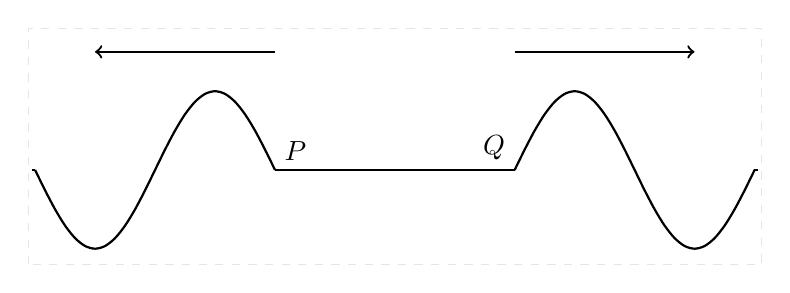
\begin{tikzpicture}[x=0.04\columnwidth]
                \draw[dashed,white!90!black] (-9.6,-1.2) rectangle (9.6,1.8);
                %% left
                \draw[thick] (0,0) -- (-3.14,0);
                \draw[domain=0:2*pi,smooth,thick] plot (\x-9.42, {-1*sin(\x r)});
                \draw[thick] (-9.42,0) -- (-9.50,0);
                \draw[thick,->] (-3.14,1.5) -- (-7.85,1.5);
                %% right
                \draw[thick] (0,0) -- (3.14,0);
                \draw[domain=0:2*pi,smooth,thick] plot (\x+3.14, {sin(\x r)});
                \draw[thick] (9.42,0) -- (9.50,0);
                \draw[thick,->] (3.14,1.5) -- (7.85,1.5);
                %% P and Q
                \node[anchor=south west] at (-3.14,0) {$P$};
                \node[anchor=south east] at (+3.14,0) {$Q$};
            \end{tikzpicture}
        }
        %% B
        \wrongchoice{
            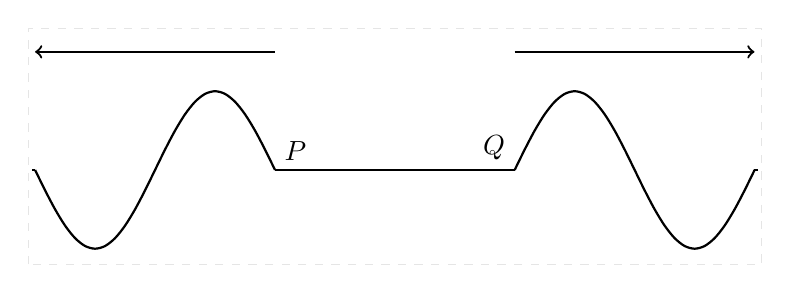
\begin{tikzpicture}[x=0.04\columnwidth]
                \draw[dashed,white!90!black] (-9.6,-1.2) rectangle (9.6,1.8);
                %% left
                \draw[thick] (0,0) -- (-3.14,0);
                \draw[domain=0:2*pi,smooth,thick] plot (\x-9.42, {-1*sin(\x r)});
                \draw[thick] (-9.42,0) -- (-9.50,0);
                \draw[thick,->] (-3.14,1.5) -- (-9.42,1.5);
                %% right
                \draw[thick] (0,0) -- (3.14,0);
                \draw[domain=0:2*pi,smooth,thick] plot (\x+3.14, {sin(\x r)});
                \draw[thick] (9.42,0) -- (9.50,0);
                \draw[thick,->] (3.14,1.5) -- (9.42,1.5);
                %% P and Q
                \node[anchor=south west] at (-3.14,0) {$P$};
                \node[anchor=south east] at (+3.14,0) {$Q$};
            \end{tikzpicture}
        }
        \wrongchoice{
            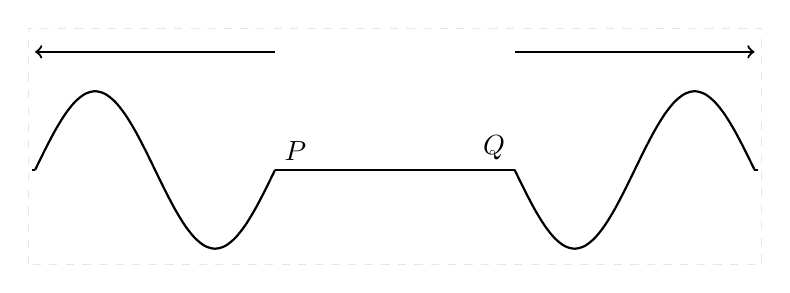
\begin{tikzpicture}[x=0.04\columnwidth]
                \draw[dashed,white!90!black] (-9.6,-1.2) rectangle (9.6,1.8);
                %% left
                \draw[thick] (0,0) -- (-3.14,0);
                \draw[domain=0:2*pi,smooth,thick] plot (\x-9.42, {1*sin(\x r)});
                \draw[thick] (-9.42,0) -- (-9.50,0);
                \draw[thick,->] (-3.14,1.5) -- (-9.42,1.5);
                %% right
                \draw[thick] (0,0) -- (3.14,0);
                \draw[domain=0:2*pi,smooth,thick] plot (\x+3.14, {-1*sin(\x r)});
                \draw[thick] (9.42,0) -- (9.50,0);
                \draw[thick,->] (3.14,1.5) -- (9.42,1.5);
                %% P and Q
                \node[anchor=south west] at (-3.14,0) {$P$};
                \node[anchor=south east] at (+3.14,0) {$Q$};
            \end{tikzpicture}
        }
    \end{choices}
\end{question}
}
\end{comment}

\element{project}{
\begin{question}{testA-Q12}
    The prediction of a ``heat death'' is based on the principle which states that:
    \begin{choices}
        \wrongchoice{the law of conservation of energy applies only to closed systems.}
        \wrongchoice{at some time in the future, the energy of the universe will become zero.}
      \correctchoice{all bodies in the universe will eventually reach the same temperature by exchanging heat with each other.}
        \wrongchoice{it is impossible to think of a system in which energy is completely conserved.}
    \end{choices}
\end{question}
}

\element{project}{
\begin{question}{testA-Q13}
    The law of normal distribution applies in \emph{all except one} of the following cases.
    Which one is the exception?
    \begin{choices}
        \wrongchoice{the heights of a large number of 25-year-old maple trees in a certain forest}
      \correctchoice{the speed of a falling object measured at many different times during the object's fall}
        \wrongchoice{the scores on a test taken by a large number of students.}
    \end{choices}
\end{question}
}

\newcommand{\testAQfourteenA}{
\begin{tikzpicture}
    \begin{axis}[
        axis y line=left,
        axis x line=bottom,
        axis line style={->},
        xlabel={time},
        xtick=\empty,
        ylabel={},
        ytick=\empty,
        xmin=0,xmax=8,
        ymin=0,ymax=10,
        width=1.0\columnwidth,
        very thin,
    ]
    \addplot[line width=1pt,mark=\empty]
        plot coordinates { (0,5) (2,9) (4,4) (6,9) (8,5) };
    \end{axis}
\end{tikzpicture}
}

\newcommand{\testAQfourteenB}{
\begin{tikzpicture}
    \begin{axis}[
        axis y line=left,
        axis x line=bottom,
        axis line style={->},
        xlabel={time},
        xtick=\empty,
        ylabel={},
        ytick=\empty,
        xmin=0,xmax=8,
        ymin=0,ymax=10,
        width=1.0\columnwidth,
        very thin,
    ]
    \addplot[line width=1pt,mark=\empty]
        plot coordinates { (0,5) (2,1) (4,5) (6,1) (8,5) };
    \end{axis}
\end{tikzpicture}
}

\newcommand{\testAQfourteenC}{
\begin{tikzpicture}
    \begin{axis}[
        axis y line=left,
        axis x line=bottom,
        axis line style={->},
        xlabel={time},
        xtick=\empty,
        ylabel={},
        ytick=\empty,
        xmin=0,xmax=10,
        ymin=0,ymax=10,
        width=1.0\columnwidth,
        very thin,
    ]
    \addplot[line width=1pt,mark=\empty]
        plot coordinates { (0,5) (10,5) };
    \end{axis}
\end{tikzpicture}
}

\newcommand{\testAQfourteenD}{
\begin{tikzpicture}
    \begin{axis}[
        axis y line=left,
        axis x line=bottom,
        axis line style={->},
        xlabel={time},
        xtick=\empty,
        ylabel={},
        ytick=\empty,
        xmin=0,xmax=8,
        ymin=0,ymax=6,
        width=1.0\columnwidth,
        very thin,
    ]
    %% NOTE: more accurately \sin^2
    %% NOTE: v(t) = A \sin \omega t
    %% NOTE: KE \propto v(t)^2
    \draw[line width=1pt] (axis cs:0,3) arc (180:0:2) arc(180:0:2);
    \end{axis}
\end{tikzpicture}
}

\newcommand{\testAQfourteenE}{
\begin{tikzpicture}
    \begin{axis}[
        axis y line=left,
        axis x line=bottom,
        axis line style={->},
        xlabel={time},
        xtick=\empty,
        ylabel={},
        ytick=\empty,
        xmin=0,xmax=8,
        ymin=0,ymax=6,
        width=1.0\columnwidth,
        very thin,
    ]
    %% NOTE: more accurately \sin^2
    \draw[line width=1pt] (axis cs:0,3) arc (180:360:2) arc(180:360:2);
    \end{axis}
\end{tikzpicture}
}

\element{project}{
\begin{question}{testA-Q14}
    %The following graphs refer to questions 14 and 15.
    At time $t=$zero a pendulum is set into motion by
        releasing the pendulum bob at a certain height.
    Which of the graphs best represents the variation
        of the bob's kinetic energy with time?
    \begin{multicols}{2}
    \begin{choices}
        \AMCboxDimensions{down=-2.5em}
        \wrongchoice{\testAQfourteenA}
        \wrongchoice{\testAQfourteenB}
        \wrongchoice{\testAQfourteenC}
      \correctchoice{\testAQfourteenD}
        \wrongchoice{\testAQfourteenE}
    \end{choices}
    \end{multicols}
\end{question}
}

\element{project}{
\begin{question}{testA-Q15}
    %The following graphs refer to questions 14 and 15.
    At time $t=$zero a pendulum is set into motion by
        releasing the pendulum bob at a certain height.
    Which of the graphs best represents the variation
        of potential energy with time?
    \begin{multicols}{2}
    \begin{choices}
        \AMCboxDimensions{down=-2.5em}
        \wrongchoice{\testAQfourteenA}
        \wrongchoice{\testAQfourteenB}
        \wrongchoice{\testAQfourteenC}
        \wrongchoice{\testAQfourteenD}
      \correctchoice{\testAQfourteenE}
    \end{choices}
    \end{multicols}
\end{question}
}


%% Test B
%%--------------------
\element{project}{
\begin{question}{testB-Q01}
    An object at rest may have a non-zero amount of:
    \begin{multicols}{2}
    \begin{choices}
        \wrongchoice{momentum.}
      \correctchoice{energy.}
        \wrongchoice{speed.}
        \wrongchoice{velocity.}
    \end{choices}
    \end{multicols}
\end{question}
}

\element{project}{
\begin{question}{testB-Q02}
    \emph{All except one} of the following can be
        adequately described by Newtonian mechanics.
    Which one is the exception?
    \begin{choices}
        \wrongchoice{the motion of a flare dropped from an airplane}
        \wrongchoice{the relationships between observable properties of gases}
        \wrongchoice{the sizes and speeds of molecules in a gas}
      \correctchoice{the motions of atoms inside molecules}
    \end{choices}
\end{question}
}

\element{project}{
\begin{question}{testB-Q03}
    The first law of thermodynamics is a statement of
    \begin{choices}
      \correctchoice{the law of conservation of energy.}
        \wrongchoice{the law of conservation of momentum.}
        \wrongchoice{the law of conservation of mass.}
        \wrongchoice{Newton's law of action and reaction.}
        \wrongchoice{Galileo's law of motion.}
    \end{choices}
\end{question}
}

\newcommand{\testBQfourA}{
\begin{tikzpicture}
    \begin{axis}[
        axis y line=left,
        axis x line=middle,
        axis line style={->},
        xlabel={time},
        xtick=\empty,
        x label style={anchor=north east},
        ylabel={},
        ytick=\empty,
        xmin=0,xmax=11,
        ymin=-3,ymax=6,
        width=1.0\columnwidth,
        very thin,
    ]
    \draw[line width=1pt] (axis cs:0,5)
        to[out=0,in=180] (axis cs:2,5)
        to[out=0,in=180] (axis cs:5,0)
        to[out=0,in=180] (axis cs:7,2)
        to[out=0,in=180] (axis cs:10,2);
    \end{axis}
\end{tikzpicture}
}

\newcommand{\testBQfourB}{
\begin{tikzpicture}
    \begin{axis}[
        axis y line=left,
        axis x line=middle,
        axis line style={->},
        xlabel={time},
        xtick=\empty,
        x label style={anchor=north east},
        ylabel={},
        ytick=\empty,
        xmin=0,xmax=11,
        ymin=-3,ymax=6,
        width=1.0\columnwidth,
        very thin,
    ]
    \draw[line width=1pt] (axis cs:0,2)
        to[out=0,in=180] (axis cs:3,2)
        to[out=0,in=180] (axis cs:5,5)
        to[out=0,in=180] (axis cs:7,2)
        to[out=0,in=180] (axis cs:10,2);
    \end{axis}
\end{tikzpicture}
}

\newcommand{\testBQfourC}{
\begin{tikzpicture}
    \begin{axis}[
        axis y line=left,
        axis x line=middle,
        axis line style={->},
        xlabel={time},
        xtick=\empty,
        x label style={anchor=north east},
        ylabel={},
        ytick=\empty,
        xmin=0,xmax=11,
        ymin=-3,ymax=6,
        width=1.0\columnwidth,
        very thin,
    ]
    \draw[line width=1pt] (axis cs:0,2)
        to[out=0,in=180] (axis cs:3,2)
        to[out=0,in=180] (axis cs:5,0)
        to[out=0,in=180] (axis cs:7,2)
        to[out=0,in=180] (axis cs:10,2);
    \end{axis}
\end{tikzpicture}
}

\newcommand{\testBQfourD}{
\begin{tikzpicture}
    \begin{axis}[
        axis y line=left,
        axis x line=middle,
        axis line style={->},
        xlabel={time},
        xtick=\empty,
        ylabel={},
        ytick=\empty,
        xmin=0,xmax=11,
        ymin=-3,ymax=6,
        width=1.0\columnwidth,
        very thin,
        clip=false,
    ]
    \draw[line width=1pt] (axis cs:0,3)
        to[out=0,in=180] (axis cs:3,3)
        to[out=0,in=180] (axis cs:5,0)
        to[out=0,in=180] (axis cs:7,-3)
        to[out=0,in=180] (axis cs:10,-3);
    \end{axis}
\end{tikzpicture}
}


\element{project}{
\begin{question}{testB-Q04}
    A ball is thrown against a wall from which it rebounds.
    %% Start question
    Which of the below graphs could best represent the kinetic energy of the ball,
        assuming an elastic collision.
    (\emph{Note:} An elastic collision is one in which the kinetic energy is the same before and after the collision.)
    \begin{multicols}{2}
    \begin{choices}
        %% NOTE: finish
        \AMCboxDimensions{down=-2.5em}
        \wrongchoice{\testBQfourA}
        \wrongchoice{\testBQfourB}
      \correctchoice{\testBQfourC}
        \wrongchoice{\testBQfourD}
    \end{choices}
    \end{multicols}
\end{question}
}

\element{project}{
\begin{question}{testB-Q05}
    %Questions 4 to 7 refer to the following graphs.
    A ball is thrown against a wall from which it rebounds.
    %% Start question
    Which of the below graphs could best represent the kinetic energy of the ball,
        if the collision is partly elastic.
    (\emph{Note:} An elastic collision is one in which the kinetic energy is the same before and after the collision.)
    \begin{multicols}{2}
    \begin{choices}
        \AMCboxDimensions{down=-2.5em}
      \correctchoice{\testBQfourA}
        \wrongchoice{\testBQfourB}
        \wrongchoice{\testBQfourC}
        \wrongchoice{\testBQfourD}
    \end{choices}
    \end{multicols}
\end{question}
}

\element{project}{
\begin{question}{testB-Q06}
    %Questions 4 to 7 refer to the following graphs.
    A ball is thrown against a wall from which it rebounds.
    %% Start question
    Which of the below graphs could best represent the
        the magnitude of the ball's velocity during an elastic collision.
    (\emph{Note:} An elastic collision is one in which the kinetic energy is the same before and after the collision.)
    \begin{multicols}{2}
    \begin{choices}
        \AMCboxDimensions{down=-2.5em}
        \wrongchoice{\testBQfourA}
        \wrongchoice{\testBQfourB}
      \correctchoice{\testBQfourC}
        \wrongchoice{\testBQfourD}
    \end{choices}
    \end{multicols}
\end{question}
}

\element{project}{
\begin{question}{testB-Q07}
    %Questions 4 to 7 refer to the following graphs.
    A ball is thrown against a wall from which it rebounds.
    %% Start question
    Which of the below graphs could best represent the
        the magnitude of the ball's velocity during a partly elastic collision.
    (\emph{Note:} An elastic collision is one in which the kinetic energy is the same before and after the collision.)
    \begin{multicols}{2}
    \begin{choices}
        \AMCboxDimensions{down=-2.5em}
      \correctchoice{\testBQfourA}
        \wrongchoice{\testBQfourB}
        \wrongchoice{\testBQfourC}
        \wrongchoice{\testBQfourD}
    \end{choices}
    \end{multicols}
\end{question}
}

\begin{comment}
\element{project}{
\begin{question}{testB-Q08}
    %Questions 8 to 13 refer to pictures of water ripples.
    %Use the following key to answer questions 8 to 13.
    Below is a picture of water ripples.
    \begin{center}
        %% NOTE: insert picture
    \end{center}
    Which of the below is illustrated by the picture above?
    \begin{choices}
        \wrongchoice{diffraction}
        \wrongchoice{refraction}
        \wrongchoice{reflection}
        \wrongchoice{interference}
    \end{choices}
\end{question}
}

\element{project}{
\begin{question}{testB-Q09}
    Below is a picture of water ripples.
    \begin{center}
        %% NOTE: insert picture
    \end{center}
    Which of the below is illustrated by the picture above?
    \begin{choices}
        \wrongchoice{diffraction}
        \wrongchoice{refraction}
        \wrongchoice{reflection}
        \wrongchoice{interference}
    \end{choices}
\end{question}
}

\element{project}{
\begin{question}{testB-Q10}
    Below is a picture of water ripples.
    \begin{center}
        %% NOTE: insert picture
    \end{center}
    Which of the below is illustrated by the picture above?
    \begin{choices}
        \wrongchoice{diffraction}
        \wrongchoice{refraction}
        \wrongchoice{reflection}
        \wrongchoice{interference}
    \end{choices}
\end{question}
}
\end{comment}

%% NOTE: duplicate of testA-Q13
\element{project}{
\begin{question}{testB-Q11}
    The law of normal distribution applies in \emph{all except one}
        of the following cases.
    Which one is the exception?
    \begin{choices}
        \wrongchoice{the heights of a large number of 25 year old maple trees in a certain forest}
      \correctchoice{the speed of a falling object measured at many different times during the object's fall}
        \wrongchoice{the scores on a test taken by a large number of students.}
    \end{choices}
\end{question}
}

\element{project}{
\begin{question}{testB-Q12}
    The second law of thermodynamics suggests that:
    \begin{choices}
      \correctchoice{energy tends to transform itself into less useful forms.}
        \wrongchoice{the usual order of natural processes is from disorder to order.}
        \wrongchoice{all natural processes are reversible.}
        \wrongchoice{it is possible to determine the motion of an individual molecule in a gas.}
    \end{choices}
\end{question}
}

\element{project}{
\begin{question}{testB-Q13}
    Even though one may listen to a band from a considerable distance,
        the sound of the piccolo and that of the tuba do not get
        ``out of step'' with each other.
    This is evidence that in this situation sound waves:
    \begin{choices}
      \correctchoice{travel at the same speed for all frequencies.}
        \wrongchoice{are not polarized.}
        \wrongchoice{are longitudinal.}
        \wrongchoice{tend to be sinusoidal.}
        \wrongchoice{travel at a slower speed than light.}
    \end{choices}
\end{question}
}

\element{project}{
\begin{question}{testB-Q14}
    All bodies contain electrical charge
        (which comes in two varieties, positive and negative).
    A law of conservation of charge applies.
    Which of the following might be a consequence or statement of that law?
    \begin{choices}
        \wrongchoice{Charge is rare and must be used carefully.}
        \wrongchoice{If an object with a net positive charge explodes, each of the pieces must have a net positive charge.}
      \correctchoice{The total net charge in an isolated system does not change with time.}
    \end{choices}
\end{question}
}

%% NOTE: duplicate of testA-Q12
\element{project}{
\begin{question}{testB-Q15}
    The prediction of a ``heat death'' is based on the principle which states that:
    \begin{choices}
        \wrongchoice{the law of conservation of energy applies only to closed systems. }
        \wrongchoice{at some time in the future, the energy of the universe will become zero. }
      \correctchoice{all bodies in the universe will eventually reach the same temperature by exchanging heat with each other. }
        \wrongchoice{it is impossible to think of a system in which energy is completely conserved. }
    \end{choices}
\end{question}
}


%% Test C
%%--------------------
\element{project}{
\begin{question}{testC-Q01}
    Which of the following is a vector quantity?
    \begin{multicols}{2}
    \begin{choices}
      \correctchoice{momentum}
        \wrongchoice{kinetic energy}
        \wrongchoice{work}
        \wrongchoice{heat}
        \wrongchoice{temperature}
    \end{choices}
    \end{multicols}
\end{question}
}

\element{project}{
\begin{question}{testC-Q02}
    A \SI{10}{\kilo\gram} weight is dropped from a height of 3 meters.
    Just before striking the ground the weight's kinetic energy will be about:
    \begin{multicols}{2}
    \begin{choices}
        \wrongchoice{\SI{3}{\joule}}
        \wrongchoice{\SI{30}{\joule}}
      \correctchoice{\SI{300}{\joule}}
        \wrongchoice{\SI{3000}{\joule}}
    \end{choices}
    \end{multicols}
\end{question}
}

\element{project}{
\begin{question}{testC-Q03}
    A number of the examples of the energy concept make
        use of ``frictionless'' systems.
    Why is this done?
    \begin{choices}
        \wrongchoice{Most systems are frictionless.}
        \wrongchoice{Total energy is not conserved when friction is present.}
        \wrongchoice{Friction is not as meaningful a concept as energy.}
        \wrongchoice{Friction is not present in outer space.}
      \correctchoice{It is often possible to get useful answers by ignoring friction.}
    \end{choices}
\end{question}
}

\element{project}{
\begin{question}{testC-Q04}
    Which one of the following is most nearly an ``elastic'' collision?
    \begin{choices}
        \wrongchoice{two railway cars coupling}
        \wrongchoice{an automobile collision}
      \correctchoice{two billiard balls colliding}
        \wrongchoice{an apple dropped on the ground}
        \wrongchoice{a hammer hitting a nail into wood}
    \end{choices}
\end{question}
}

\element{project}{
\begin{question}{testC-Q05}
    When the displacement pattern of a transverse
        wave lies in a single plane, the wave is said to be:
    \begin{choices}
        \wrongchoice{reflected.}
      \correctchoice{polarized.}
        \wrongchoice{diffracted.}
        \wrongchoice{refracted.}
    \end{choices}
\end{question}
}

\element{project}{
\begin{question}{testC-Q06}
    Two steel balls collide elastically.
    \begin{choices}
        \wrongchoice{Momentum is the same before and after the collision, but kinetic energy is not.}
      \correctchoice{Momentum and kinetic energy are the same before and after the collision.}
        \wrongchoice{The temperature of both balls will increase.}
        \wrongchoice{The balls will be permanently deformed.}
        \wrongchoice{The balls will stick together.}
    \end{choices}
\end{question}
}

%% NOTE: duplicate of testB-Q02
\element{project}{
\begin{question}{testC-Q07}
    \emph{All except one} of the following can be
        adequately described by Newtonian mechanics.
    Which one is the exception?
    \begin{choices}
        \wrongchoice{the motion of a flare dropped from an airplane}
        \wrongchoice{the relationships between observable properties of gases}
        \wrongchoice{the sizes and speeds of molecules in a gas}
      \correctchoice{the motions of atoms inside molecules}
    \end{choices}
\end{question}
}

%% NOTE: duplicate of testA-Q13 and testB-Q11
\element{project}{
\begin{question}{testC-Q08}
    The law of normal distribution applies in \emph{all except one}
        of the following cases.
    Which one is the exception?
    \begin{choices}
        \wrongchoice{the heights of a large number of 25-year-old maple trees in a certain forest}
      \correctchoice{the speed of a falling object measured at many different times during the object's fall}
        \wrongchoice{the scores on a test written by a large number of students}
    \end{choices}
\end{question}
}

%% NOTE: duplicate of testB-Q12
\element{project}{
\begin{question}{testC-Q09}
    The second law of thermodynamics suggests that:
    \begin{choices}
      \correctchoice{energy tends to transform itself into less useful forms.}
        \wrongchoice{the usual order of natural processes is from disorder to order.}
        \wrongchoice{all natural processes are reversible.}
        \wrongchoice{it is possible to determine the motion of individual molecules in a gas.}
    \end{choices}
\end{question}
}

\element{project}{
\begin{question}{testC-Q10}
    Some men feeling the need for exercise organize a baseball game.
    The first batter hits a waist-high pitch over the center fielder's head.
    %% Start question
    If air resistance is negligible,
        only one of the following statements about the
        ball during its flight is \emph{false}.
    Which one?
    \begin{choices}
        \wrongchoice{The higher the ball goes, the greater its gravitational potential energy.}
        \wrongchoice{The horizontal component of the ball's velocity is constant.}
        \wrongchoice{The total energy of the ball is constant.}
        %% NOTE: momentum is a vector quantity
      \correctchoice{The momentum of the ball is constant.}
    \end{choices}
\end{question}
}

\newcommand{\testCQelevenW}{
\begin{tikzpicture}
    %% ground
    \draw (0,0) -- (5,0);
    \node[anchor=north,pattern=north east lines,minimum width=5cm,minimum height=0.05cm] at (2.5,0) {};
    %% path
    \draw[thick] (0.25,0) -- (1.5,2) node[anchor=east] {$W$};
    \draw[thick] (1.5,2) -- (2.75,0.5) node[anchor=west] {$B$};
\end{tikzpicture}
}

\newcommand{\testCQelevenX}{
\begin{tikzpicture}
    %% ground
    \draw (0,0) -- (5,0);
    \node[anchor=north,pattern=north east lines,minimum width=5cm,minimum height=0.05cm] at (2.5,0) {};
    %% path
    \draw[thick] (0.25,0) -- (1.5,2) node[anchor=east] {$X$};
    \draw[thick] (1.5,2) parabola bend (2.75,0.5)  (2.75,0.5) node[anchor=west] {$B$};
\end{tikzpicture}
}

\newcommand{\testCQelevenY}{
\begin{tikzpicture}
    %% ground
    \draw (0,0) -- (5,0);
    \node[anchor=north,pattern=north east lines,minimum width=5cm,minimum height=0.05cm] at (2.5,0) {};
    %% path
    \draw[thick] (0.25,0) -- (1.5,2) node[anchor=east] {$Y$};
    \draw[thick] (1.5,2) parabola bend (1.5,2) (2.75,0.5) node[anchor=west] {$B$};
\end{tikzpicture}
}

\newcommand{\testCQelevenZ}{
\begin{tikzpicture}
    %% ground
    \draw (0,0) -- (5,0);
    \node[anchor=north,pattern=north east lines,minimum width=5cm,minimum height=0.05cm] at (2.5,0) {};
    %% path
    \draw[thick] (0.25,0) -- (1.5,2) node[anchor=east] {$Z$};
    \draw[thick] (1.5,2) -- (4.75,0.5) node[anchor=west] {$B$};
\end{tikzpicture}
}

\element{project}{
\begin{questionmult}{testC-Q11}
    A girl wants to slide down a playground slide so that she will
        have the greatest possible speed when she reaches the bottom (point $B$).
    Which of the following frictionless slides should she choose?
    (Points $W$, $X$, $Y$, $Z$ are all two meters above the ground,
        and point $B$ is 0.5 meters above the ground.)
    \begin{choices}
        \AMCboxDimensions{down=-1em}
        \correctchoice{\testCQelevenW}
        \correctchoice{\testCQelevenX}
        \correctchoice{\testCQelevenY}
        \correctchoice{\testCQelevenZ}
        %\wrongchoice{slide $W$}
        %\wrongchoice{slide $X$}
        %\wrongchoice{slide $Y$}
        %\wrongchoice{slide $Z$}
        %\correctchoice{The speed at $B$ will be the same for each.}
    \end{choices}
\end{questionmult}
}

\element{project}{
\begin{question}{testC-Q12}
    Leibniz's \emph{vis viva} most closely resembles:
    \begin{choices}
        \wrongchoice{potential energy.}
      \correctchoice{kinetic energy.}
        \wrongchoice{heat.}
        \wrongchoice{velocity.}
        \wrongchoice{momentum.}
    \end{choices}
\end{question}
}

\begin{comment}
%% NOTE: duplicate of testB-Q08
\element{project}{
\begin{question}{testC-Q13}
    Below is a picture of water ripples.
    \begin{center}
        %% NOTE: insert picture
    \end{center}
    Which of the below is illustrated by the picture above?
    \begin{choices}
        \wrongchoice{diffraction}
        \wrongchoice{refraction}
        \wrongchoice{reflection}
        \wrongchoice{interference}
    \end{choices}
\end{question}
}

%% NOTE: duplicate of testB-Q09
\element{project}{
\begin{question}{testC-Q14}
    Below is a picture of water ripples.
    \begin{center}
        %% NOTE: insert picture
    \end{center}
    Which of the below is illustrated by the picture above?
    \begin{choices}
        \wrongchoice{diffraction}
        \wrongchoice{refraction}
        \wrongchoice{reflection}
        \wrongchoice{interference}
    \end{choices}
\end{question}
}

%% NOTE: duplicate of testB-Q10
\element{project}{
\begin{question}{testC-Q15}
    Below is a picture of water ripples.
    \begin{center}
        %% NOTE: insert picture
    \end{center}
    Which of the below is illustrated by the picture above?
    \begin{choices}
        \wrongchoice{diffraction}
        \wrongchoice{refraction}
        \wrongchoice{reflection}
        \wrongchoice{interference}
    \end{choices}
\end{question}
}
\end{comment}

\element{project}{
\begin{question}{testC-Q16}
    %Questions 16 and 17 refer to the following statement:
    A \SI{0.1}{\kilo\gram} snowball strikes a 0.9 kilogram
        stationary skateboard and sticks to it.
    At the instant of impact, the snowball has a velocity of
        \SI{18}{\meter\per\second} in the horizontal direction.
    (Assume that the skateboard is on a perfectly horizontal stretch
        of ground and that it moves without friction.) \\[0.5\baselineskip]
    %% NOTE: insert graphic
    After collision, the skateboard and snowball move horizontally with a velocity of:
    \begin{multicols}{2}
    \begin{choices}
        \wrongchoice{\SI{1.8}{\meter\per\second}}
        \wrongchoice{\SI{2}{\meter\per\second}}
        \wrongchoice{\SI{16.2}{\meter\per\second}}
        \wrongchoice{\SI{18}{\meter\per\second}}
        \wrongchoice{\SI{180}{\meter\per\second}}
    \end{choices}
    \end{multicols}
\end{question}
}

\element{project}{
\begin{question}{testC-Q17}
    %Questions 16 and 17 refer to the following statement:
    A \SI{0.1}{\kilo\gram} snowball strikes a 0.9 kilogram
        stationary skateboard and sticks to it.
    At the instant of impact, the snowball has a velocity of
        \SI{18}{\meter\per\second} in the horizontal direction.
    (Assume that the skateboard is on a perfectly horizontal stretch
        of ground and that it moves without friction.) \\[0.5\baselineskip]
    \begin{center}
    \begin{tikzpicture}
        %% NOTE: TODO: insert graphic
    \end{tikzpicture}
    \end{center}
    Kinetic energy is not conserved in the above collision because:
    \begin{choices}
        \wrongchoice{the system is not closed.}
        \wrongchoice{the collision is not perfectly elastic.}
        \wrongchoice{momentum and energy cannot both be conserved in a collision.}
        \wrongchoice{the law of conservation of energy does not hold for a frictionless system.}
        \wrongchoice{heat cannot flow from a cold object to a hot object.}
    \end{choices}
\end{question}
}

\element{project}{
\begin{question}{testC-Q18}
    An object is hung on a vertical spring and allowed to oscillate up and down.
    At any instant the system's total energy is:
    \begin{choices}
      \correctchoice{KE + PE\textsubscript{elastic} + PE\textsubscript{gravitational}}
        \wrongchoice{KE + PE\textsubscript{elastic}}
        \wrongchoice{KE + PE\textsubscript{gravitational}}
        \wrongchoice{PE\textsubscript{elastic} + PE\textsubscript{gravitational}}
        \wrongchoice{KE}
    \end{choices}
\end{question}
}

\element{project}{
\begin{question}{testC-Q19}
    Which one of the following is transferred from one place to another by a propagating wave?
    \begin{multicols}{2}
    \begin{choices}
        \wrongchoice{mass}
      \correctchoice{energy}
        \wrongchoice{time}
        \wrongchoice{velocity}
    \end{choices}
    \end{multicols}
\end{question}
}

\element{project}{
\begin{question}{testC-Q20}
    A body's momentum is defined as the body's mass times its velocity.
    The mks (meter kilogram second) unit of momentum is:
    \begin{choices}
        \wrongchoice{kilogram meter (\si{\kilo\gram\meter}).}
      \correctchoice{kilogram meter per second (\si{\kilo\gram\meter\per\second}).}
        \wrongchoice{kilogram meter squared per second squared (\si{\kilo\gram\meter\squared\per\second\squared}).}
        \wrongchoice{kilogram squared meter per second (\si{\kilo\gram\squared\meter\per\second}).}
        \wrongchoice{none of the provided.}
    \end{choices}
\end{question}
}

%% NOTE: duplicate of testA-Q06
\element{project}{
\begin{question}{testC-Q21}
    Below are the names of scientists who made early
        significant contributions to the study of thermodynamics.
    Which statement best describe the contributions of
        James Prescott Joule?
    \begin{choices}
        \wrongchoice{The pressure of a gas is proportional to the square of the speed of its molecules.}
      \correctchoice{Heat is a form of energy.}
        \wrongchoice{The speeds of molecules in a gas follow a statistical law.}
        \wrongchoice{In an elastic collision, momentum is conserved.}
        \wrongchoice{The process of equalization of temperatures by the flow of heat from hot to cold bodies is always taking place in nature.}
    \end{choices}
\end{question}
}

%% NOTE: duplicate of testA-Q07
\element{project}{
\begin{question}{testC-Q22}
    Below are the names of scientists who made early
        significant contributions to the study of thermodynamics.
    Which statement best describe the contributions of
        Nicolas L\'{e}onard Sadi Carnot?
    \begin{choices}
        \wrongchoice{The pressure of a gas is proportional to the square of the speed of its molecules.}
        \wrongchoice{Heat is a form of energy.}
        \wrongchoice{The speeds of molecules in a gas follow a statistical law.}
        \wrongchoice{In an elastic collision, momentum is conserved.}
      \correctchoice{The process of equalization of temperatures by the flow of heat from hot to cold bodies is always taking place in nature.}
    \end{choices}
\end{question}
}

%% NOTE: duplicate of testA-Q08
\element{project}{
\begin{question}{testC-Q23}
    Below are the names of scientists who made early
        significant contributions to the study of thermodynamics.
    Which statement best describe the contributions of
        James Clerk Maxwell?
    \begin{choices}
        \wrongchoice{The pressure of a gas is proportional to the square of the speed of its molecules.}
        \wrongchoice{Heat is a form of energy.}
      \correctchoice{The speeds of molecules in a gas follow a statistical law.}
        \wrongchoice{In an elastic collision, momentum is conserved.}
        \wrongchoice{The process of equalization of temperatures by the flow of heat from hot to cold bodies is always taking place in nature.}
    \end{choices}
\end{question}
}

%% NOTE: duplicate of testA-Q09
\element{project}{
\begin{question}{testC-Q24}
    A girl lifts a bowling ball from the floor and places it on a rack.
    If you know the weight of the ball,
        what else must you know in order to calculate the work she does on the ball?
    \begin{choices}
        \wrongchoice{mass of the ball}
        %% NOTE: changed ag to g
        \wrongchoice{value of $g$}
      \correctchoice{height of the rack}
        \wrongchoice{the time required}
        \wrongchoice{nothing else}
    \end{choices}
\end{question}
}

\element{project}{
\begin{question}{testC-Q25}
    %% Johann Wolfgang von Goethe's
    \emph{All except one} of the following are in agreement with Johann Goethe's nature-philosophy.
    Which one is the exception?
    \begin{choices}
      \correctchoice{The methods of mechanistic science---for example, mathematical analysis and experimentation---give the wrong idea of nature.}
        \wrongchoice{Nature as it really is can be understood by direct observation.}
        \wrongchoice{One should search for the inner meaning of nature.}
        \wrongchoice{Laws that are practical and quantitative can best describe nature.}
    \end{choices}
\end{question}
}

\element{project}{
\begin{question}{testC-Q26}
    The kinetic energy of an object is increased the most by doubling its:
    \begin{multicols}{2}
    \begin{choices}
        \wrongchoice{mass.}
        \wrongchoice{temperature.}
        \wrongchoice{volume.}
        \wrongchoice{density.}
      \correctchoice{speed.}
    \end{choices}
    \end{multicols}
\end{question}
}

%% NOTE: duplicate of testB-Q03
\element{project}{
\begin{question}{testC-Q27}
    The first law of thermodynamics is a statement of:
    \begin{choices}
      \correctchoice{the law of conservation of energy,}
        \wrongchoice{the law of conservation of momentum.}
        \wrongchoice{the law of conservation of mass,}
        \wrongchoice{Newton's law of action and reaction,}
        \wrongchoice{Galileo's law of motion.}
    \end{choices}
\end{question}
}

\begin{comment}
%% NOTE: duplicate of testA-Q10
\element{project}{
\begin{question}{testC-Q28}
    %Questions 28 and 29 refer to the following statement and diagram.
    Two wave pulses, each of length 1, are traveling toward each other
        along a rope as illustrated in the diagram below. \\[0.5\baselineskip]
    %% NOTE: finish
    At the instant that both waves are entirely in the region
        between $P$ and $Q$, the shape of the rope will be:
    \begin{choices}
        \wrongchoice{
            \begin{tikzpicture}
            \end{tikzpicture}
        }
    \end{choices}
\end{question}
}

%% NOTE: duplicate of testA-Q11
\element{project}{
\begin{question}{testC-Q29}
    %Questions 28 and 29 refer to the following statement and diagram.
    Two wave pulses, each of length 1, are traveling toward each other
        along a rope as illustrated in the diagram below. \\[0.5\baselineskip]
    %% start question
    Just after both wave pulses have passed the region between $P$ and $Q$,
        the shape of the rope will be:
    \begin{choices}
        \wrongchoice{
            \begin{tikzpicture}
            \end{tikzpicture}
        }
    \end{choices}
\end{question}
}
\end{comment}

%% NOTE: duplicate of testB-Q04
\element{project}{
\begin{question}{testC-Q30}
    %% Items 30 to 33 refer to the following graphs.
    A ball is thrown against a wall from which it rebounds.
    %% Start question
    Which of the below graphs could best represent the kinetic energy of the ball,
        assuming an elastic collision.
    (\emph{Note:} An elastic collision is one in which the kinetic energy is the same before and after the collision.)
    \begin{multicols}{2}
    \begin{choices}
        %% NOTE: finish
        \AMCboxDimensions{down=-2.5em}
        \wrongchoice{\testBQfourA}
        \wrongchoice{\testBQfourB}
      \correctchoice{\testBQfourC}
        \wrongchoice{\testBQfourD}
    \end{choices}
    \end{multicols}
\end{question}
}

%% NOTE: duplicate of testB-Q05
\element{project}{
\begin{question}{testC-Q31}
    %% Items 30 to 33 refer to the following graphs.
    A ball is thrown against a wall from which it rebounds.
    %% Start question
    Which of the below graphs could best represent the kinetic energy of the ball,
        if the collision is partly elastic.
    (\emph{Note:} An elastic collision is one in which the kinetic energy is the same before and after the collision.)
    \begin{multicols}{2}
    \begin{choices}
        \AMCboxDimensions{down=-2.5em}
      \correctchoice{\testBQfourA}
        \wrongchoice{\testBQfourB}
        \wrongchoice{\testBQfourC}
        \wrongchoice{\testBQfourD}
    \end{choices}
    \end{multicols}
\end{question}
}

%% NOTE: duplicate of testB-Q06
\element{project}{
\begin{question}{testC-Q32}
    %% Items 30 to 33 refer to the following graphs.
    A ball is thrown against a wall from which it rebounds.
    %% Start question
    Which of the below graphs could best represent the
        the magnitude of the ball's velocity during an elastic collision.
    (\emph{Note:} An elastic collision is one in which the kinetic energy is the same before and after the collision.)
    \begin{multicols}{2}
    \begin{choices}
        \AMCboxDimensions{down=-2.5em}
        \wrongchoice{\testBQfourA}
        \wrongchoice{\testBQfourB}
      \correctchoice{\testBQfourC}
        \wrongchoice{\testBQfourD}
    \end{choices}
    \end{multicols}
\end{question}
}

%% NOTE: duplicate of testB-Q07
\element{project}{
\begin{question}{testC-Q33}
    %% Items 30 to 33 refer to the following graphs.
    A ball is thrown against a wall from which it rebounds.
    %% Start question
    Which of the below graphs could best represent the
        the magnitude of the ball's velocity during a partly elastic collision.
    (\emph{Note:} An elastic collision is one in which the kinetic energy is the same before and after the collision.)
    \begin{multicols}{2}
    \begin{choices}
        \AMCboxDimensions{down=-2.5em}
      \correctchoice{\testBQfourA}
        \wrongchoice{\testBQfourB}
        \wrongchoice{\testBQfourC}
        \wrongchoice{\testBQfourD}
    \end{choices}
    \end{multicols}
\end{question}
}

\element{project}{
\begin{question}{testC-Q34}
    The principle of superposition states that:
    \begin{choices}
      \correctchoice{the amplitudes of waves which coincide at a point may be added.}
        \wrongchoice{the wavelength of a reflected wave equals the wavelength of the incident wave.}
        \wrongchoice{every point on a wave front may be considered to behave as a point source of waves.}
        \wrongchoice{the diffraction pattern depends on the ratio of the wavelength to the slit width.}
    \end{choices}
\end{question}
}

%% NOTE: duplicate of testA-Q12 and testB-Q15
\element{project}{
\begin{question}{testC-Q35}
    The prediction of a ``heat death'' is based on the principle which states that:
    \begin{choices}
        \wrongchoice{the law of conservation of energy applies only to closed systems.}
        \wrongchoice{at some time in the future, the energy of the universe will become zero.}
      \correctchoice{all bodies in the universe will eventually reach the same temperature by exchanging heat with each other.}
        \wrongchoice{it is impossible to think of a system in which energy is completely conserved.}
        \wrongchoice{heat must flow from a cold object to a hot object.}
    \end{choices}
\end{question}
}

%% NOTE: duplicate of testB-Q13
\element{project}{
\begin{question}{testC-Q36}
    Even though one may listen to a band from a considerable distance,
        the sound of the piccolo and that of the tuba do not get
        ``out of step'' with each other.
    This is evidence that in this situation sound waves:
    \begin{choices}
      \correctchoice{travel at the same speed for all frequencies.}
        \wrongchoice{are not polarized.}
        \wrongchoice{are longitudinal,}
        \wrongchoice{tend to be sinusoidal.}
        \wrongchoice{travel at a slower speed than light.}
    \end{choices}
\end{question}
}

\element{project}{
\begin{question}{testC-Q37}
    Two spheres of the same diameter,
        one of mass \SI{5}{\kilo\gram} and the other of mass \SI{10}{\kilo\gram},
        are dropped at the same time from the top of a tower.
    When they are \SI{1}{\meter} above the ground,
        the two spheres have the same:
    \begin{choices}
         \wrongchoice{momentum.}
         \wrongchoice{kinetic energy.}
         \wrongchoice{potential energy.}
         \wrongchoice{total mechanical energy.}
       \correctchoice{acceleration.}
    \end{choices}
\end{question}
}

\element{project}{
\begin{question}{testC-Q38}
    When a gas is held at a constant temperature, its molecules:
    \begin{choices}
      \correctchoice{have a certain constant average energy.}
        \wrongchoice{all have the same energy.}
        \wrongchoice{all have different energies that remain constant.}
    \end{choices}
\end{question}
}

\element{project}{
\begin{question}{testC-Q39}
    The unit ``horsepower'' is a measure of:
    \begin{choices}
        \wrongchoice{force.}
        \wrongchoice{work.}
        \wrongchoice{work per bushel of coal.}
      \correctchoice{work per unit time.}
        \wrongchoice{work per steam engine.}
    \end{choices}
\end{question}
}

\element{project}{
\begin{question}{testC-Q40}
    In 1620 Francis Bacon wrote:
        ``There is nothing more true in nature than the twin propositions
        that `nothing is produced from nothing' and `nothing is reduced to
        nothing' \ldots\ the sum total of matter remains unchanged,
        without increase or diminution.''
    This statement implies which of the following basic scientific principles?
    \begin{choices}
        \wrongchoice{conservation of momentum}
        \wrongchoice{conservation of vis viva}
      \correctchoice{conservation of mass}
        \wrongchoice{conservation of mechanical energy}
        \wrongchoice{conservation of charge}
    \end{choices}
\end{question}
}

\endinput

